\chapter{The ATLAS experiment at the Large Hadron Collider}
\label{chapter:ATLASDetector}

The Large Hadron Collider (LHC) is the world's highest-energy particle accelerator, designed to collide protons at a \com\ energy of \unit[14]{\tev}.
The ATLAS experiment is one of the two multi-purpose experiments that take advantage of the collisions provided by the LHC.
It has been conceived to pursuit an ambitious physics program, where the first milestone was the discovery of the Higgs boson, achieved in 2012~\cite{Aad:2012tfa,Chatrchyan:2012ufa}.
This chapter introduces CERN's accelerator complex and describes the main aspects of the ATLAS detector at the LHC.


\section{The Large Hadron Collider}
\label{sec:LHC}

The Large Hadron Collider (LHC)~\cite{Evans:2008zzb} is a circular particle accelerator installed in a \unit[27]{km} long underground tunnel, and designed to collide protons at a \com\ energy of $\sqrt{s} = \unit[14]{\TeV}$.
On the accelerator ring four detectors (ALICE~\cite{Aamodt:2008zz}, ATLAS~\cite{Aad:2008zzm}, CMS~\cite{Chatrchyan:2008aa} and LHCb~\cite{Alves:2008zz}) have been built around four different interaction points, to record and study the collisions delivered by the LHC.
ATLAS and CMS are multipurpose experiments designed to study a broad range of physics processes. The LHCb experiment is specialized in the detection of $b$-hadrons, while the ALICE collaboration focuses on the study of heavy-ion collisions.
%The LHC has been designed to collide protons at a \com\ energy of $\sqrt{s} = \unit[14]{\TeV}$.

Since 2010, the LHC has delivered proton-proton ($\pp$) collisions at a \com\ energies of \unit[7]{\TeV} and \unit[8]{\TeV} (in 2011 and 2012, respectively), about half of its nominal energy.
The LHC has produced also lead-ion (Pb-Pb) collisions with a per-nucleon \com\ energy of $\sqrt{s_{NN}} = \unit[2.76]{\TeV}$ and proton-lead (p-Pb) collisions with $\sqrt{s_{NN}} = \unit[5.02]{\TeV}$.

The protons are accelerated to the desired energy through various steps.
First, protons are extracted from the ionization of hydrogen gas and injected in the linear accelerator LINAC2, where they are accelerated to an energy of \unit[50]{\mev}.
They are then transferred into the Proton Synchrotron Booster (PSB) and accelerated up to an energy of \unit[1.4]{\gev}.
A second circular accelerator, the Proton Synchrotron (PS) brings the energy of the protons to \unit[25]{\gev} before injecting them into the Super Proton Synchrotron (SPS).
After being accelerated to \unit[450]{\gev}, the protons finally enter the two LHC beam pipes where they are boosted to energies of up to \unit[4]{\tev}.
A schematic view of the acceleration chain is shown in figure~\ref{fig:accelerator_schema}.

\begin{figure}[!tb]
  \centering
  \includegraphics[width=0.8\textwidth]{ATLASdetector/Figures/CERN_Accelerator_Complex}
  \caption{Schematic view of the CERN accelerator complex.
The four main LHC experiments are shown at the interaction points.}
  \label{fig:accelerator_schema}
\end{figure}

%The LHC ring is composed of eight arcs which are \unit[2.7]{km} long, each of which contains 154 dipole magnets, whose function is to bend the beams along the circular trajectory, and 49 quadrupole magnets, that focus the beam.
%These superconducting magnets operate at a temperature of \unit[1.9]{K}, maintained by means of liquid Helium vessels.
%Eight insertions are placed in between the arches.
%Each insertion has a specific role that characterizes its design.
%These can be injection, beam dumping, beam cleaning, or ``physics'', i.e.
%make the beams collide within an experiment.

%Maybe move this to the end of ATLAS detector, with luminosity measurement
Besides its high energy, the LHC also outperforms previous accelerators in the delivered luminosity.
The instantaneous luminosity $\InstLumi$ is defined as:

\begin{equation}
  \InstLumi = \frac{n_{b} f_{r} n_{1} n_{2}}{2\pi \Sigma_{x} \Sigma_{y}}~,
  \label{eq:InstLumiDefinition}
\end{equation} 
where $n_{1}$ and $n_{2}$ are the bunch populations (number of protons per bunch) in beams~1 and~2 respectively, $f_{r}$ is the revolution frequency of the LHC, $n_{b}$ are the number of bunch pairs colliding in each revolution, and $\Sigma_{x}$ and $\Sigma_{y}$ characterize the horizontal and vertical convolved beam widths.

The event rate of a certain process can be obtained as the product of the process \xsec\ and the instantaneous luminosity:

\begin{equation}
  \frac{dN}{dt} = \InstLumi \times \sigma~.
  \label{eq:EventRat}
\end{equation}

%This rate is then directly proportional to the the frequency $f_{r}$, the number of bunches $n_{b}$ and the number of particles in the two bunches $n_1$,$n_2$, and inversely proportional to the beam \xsec\.
The instantaneous luminosity at the ATLAS collision point is measured by dedicated subdetectors that are described in section~\ref{sec:LuminosityMeasurement}.
In 2012, the LHC reached a peak luminosity of $\unit[7.7\times 10^{33}]{cm^{-2}s^{-1}}$, which is more than half the design luminosity.
Table~\ref{tab:accelerator_parameters} shows the relevant parameters for the accelerator performance.

\begin{table}[!tb]
  \small
  \centering
  \begin{tabular}{l l l l l}
    \toprule
    \toprule
    Parameter & Design value & 2010 & 2011 & 2012 \\
    \midrule
    Beam energy (\tev) & 7 & 3.5 & 3.5 & 4 \\
    Beta function $\beta^*$ (m) & 0.55 & 2.0/3.5 & 1.5/1.0 & 0.6 \\
    Max. num. bunches/beam & 2808 & 368 & 1380 & 1380 \\
    Max. num. protons/bunch & $1.15\times10^{11}$ & $1.2\times10^{11}$ & $1.45\times10^{11}$ & $1.7\times10^{11}$ \\
    Bunch spacing (ns) & 25 & 150 & 75/50 & 50 \\
    Peak luminosity ($\unit {cm^{-2}s^{-1}}$) & $1\times10^{34}$ & $2.1\times10^{32}$ & $3.7\times10^{33}$ & $7.7\times10^{33}$ \\
    Emittance $\epsilon_n$ ($\unit{\mu rad}$) & 3.75 & 2.0 & 2.4 & 2.5 \\
    Max. $\langle \mu \rangle$ & 19 & 4 & 17 & 37 \\
    \bottomrule
    \bottomrule
  \end{tabular}
  \caption{Overview of the parameters for the LHC performance comparing the design values with their time evolution during the first long run operation in 2010-2013.}
  \label{tab:accelerator_parameters}
\end{table}

Due to the high frequency of collisions and the high density of the bunches necessary to achieve such a high luminosity, there is a non-zero probability that several events, originating from different \pp\ collisions, may occur simultaneously. These events are referred to as \textit{\pileup} and are categorized as in-time or out-of-time \pileup. In-time \pileup\ events are caused by additional interactions of protons in the same bunch collision. The out-of-time \pileup\ occurs when traces from an event in a different bunch-crossing are recorded. The mean number of interactions per bunch crossing $\langle \mu \rangle$, which is taken as measure of the \pileup\ activity, is shown in figure~\ref{fig:ATLAS_mu}.

Integrating the instantaneous luminosity over the accelerator active time (a ``fill'', when stable beams are kept colliding) the integrated luminosity is obtained, relating the total number of produced events $N_{\rm tot}$ to the \xsec:

\begin{equation}
  N_{\rm tot} = \sigma \int{\InstLumi~dt}~.
  \label{eq:IntegLumiDefinition}
\end{equation}


In 2010 ATLAS collected about $\unit[45]{pb^{-1}}$ of $\pp$ collision data at $\sqrt{s} = \unit[7]{\tev}$, and in 2011 it reached about $\unit[5]{fb^{-1}}$ at the same \com\ energy.
During 2012, the last year of data taking before the long shutdown,\footnote{LHC terminated the first phase of the $\pp$ program at the end of 2012, operated proton-heavy ion collisions for two months at the beginning of 2013 and then stopped for what is called the first ``long shutdown''.
During these two-years the accelerator and the experiments underwent substantial maintenance and upgrade works, in order to be re-operated in 2015 with higher performance at a higher \com\ energy for particle collisions.}
ATLAS collected about $\unit[20]{fb^{-1}}$ of $\pp$ collision data at $\sqrt{s}=\unit[8]{\tev}$.
Figure~\ref{fig:ATLAS_lumi} shows the luminosity recorded by ATLAS during stable beam conditions.
The difference with respect to the delivered luminosity is due to Data AcQuisition (DAQ) inefficiencies.
Of the recorded luminosity, only a part is usable for analysis, which is referred to as ``good data'', i.e.
the data that satisfy Data Quality (DQ) requirements assessed after reprocessing (see section~\ref{sec:DataQuality}).

\begin{figure}[tb!]
  \centering
    \begin{subfigure}[b]{0.49\textwidth}
  \includegraphics[width=\textwidth]{ATLASdetector/Figures/mu_2011_2012-dec}
  \caption{ }
    \label{fig:ATLAS_mu}
    \end{subfigure}
    \begin{subfigure}[b]{0.49\textwidth}
      \includegraphics[width=\textwidth]{ATLASdetector/Figures/intlumivstime2012DQ}
      \caption{}
    \label{fig:ATLAS_lumi}
    \end{subfigure}
  \caption{(a)  Mean number of interactions per beam crossing during the 2011 and 2012 LHC runs.
   (b) Total integrated luminosity versus time delivered by the LHC to ATLAS (in green), recorded by the experiment (in yellow) and selected as “good data” for analysis (in blue) for $\pp$ collisions $\sqrt{s}=\unit[8]{\tev}$ in 2012. 
}
\end{figure}

%%%%% Pile-up, has to be mentioned but this section is poor and I'm not sure it belongs here
%In order to increase the luminosity LHC operates with a high number of protons per bunch as well as a high number of bunches per beam and reduces the inter-bunch latency time. This overall defines a set of challenges that physics analysis will face associated to the high luminosity. Even at the detector design stage, the high frequency of collision environment foreseen influenced the choice of radiation resistance material for the experiment subsystems. Concerning directly the physics instead, the main problematic is pile-up.
%Pile-up events are distinguished between in-time and out-of-time pile-up. The first ones come from the multiple inelastic collisions of protons in the same bunch, as if we consider a \xsec\ of 80 mb at the nominal luminosity of 1034 cm−2s−1 the number of events per second will be something like a billion. This translates, at a collision frequency of one crossing every 25 ns, to about 20 interactions per crossing that will be detected simultaneously. A useful observable to estitage in-time pile-up is the number of reconstructed primary vertices (see Section 4.2). In addition, on the other hand, the inter-bunch time interval is so short that the electronics reading the detector might not keep up with the frequency of collisions, leading to the cumulation of events that happened in different beam crossings. This is the effect we refer to as out-of-time pile-up, and a good estimator for it is the average number of $\pp$ interactions per bunch crossing at the time of the event, < μ >,n-time and out-of-time pile-up. The first ones come from the ) nf
%with L being the average instantaneous luminosity over a time period ∆t ≫ 600 ns. The maximum values reached by the variable < μ > during the three years of data taking are reported in Table 2.1
%
%\begin{figure}[!ht]
%  \centering
%     \includegraphics[width=\textwidth]{ATLASdetector/Figures/mu_2011_2012-dec}
%     \caption{Mean number of interactions per beam crossing during 2011 and 2012 LHC runs, where $\mu = \InstLumi \times \sigma_{inelastic}/f_{r}$.}
%  \label{fig:ATLAS_pileup}
%\end{figure}

\section{The ATLAS experiment} %%%%%%%%%%%%%%%%%%%%%%% ATLAS
\label{sec:ATLAS}
ATLAS (A Toroidal LHC ApparatuS) \cite{Aad:2008zzm} is a general purpose experiment aimed at exploring a vast range of physics scenarios and designed to measure the particles produced in $\pp$ collisions at the LHC at unprecedented energies and instantaneous luminosities.
It is the biggest detector of its kind ever built (about \unit[46]{m} long, \unit[25]{m} wide and weights \unit[7000]{t}) and it is characterized by a full coverage of the space around the $\pp$ interaction point and complete containment of the particles produced in the collision. %Mentira
Different subsystems are layered concentrically one after the other, as shown in figure~\ref{fig:ATLASsketch}, each devoted to the measurement of different properties for different types of particles.
The subdetectors are grouped into three main systems:
\begin{itemize}
  \item The Inner Detector, immersed in a solenoidal magnetic field, constitutes a tracking system used to identify and measure the momenta of charged particles and to identify the interaction vertices and the displaced vertices.
  \item The Calorimeters are used to identify and measure the energy of neutral and charged particles.
They are designed to stop most types of particles, except for muons and neutrinos.
  \item The Muon Spectrometer is used to detect and measure the properties of muons.
Because muons minimally interact with the other parts of the detector and have long lifetimes, they are identified and measured in the outermost detector layer.
\end{itemize}
%Furthermore, ATLAS uses a solenoidal magnetic field in order to bend the particle trajectories in the inner detector, and a toroidal magnetic field for the muon spectrometer.

\begin{figure}[!tb]
  \begin{center}
    \includegraphics[width=\textwidth]{ATLASdetector/Figures/ATLAS_Detector.eps}
  \end{center}
  \caption{Drawing of the ATLAS detector showing the different subdetectors and the magnet systems.}
  \label{fig:ATLASsketch}
\end{figure}

\subsection{Coordinate system}
\label{subsec:Coordinate_system}

The ATLAS reference system is a cartesian right-handed coordinate system with origin at the nominal interaction point (IP) in the center of the detector.
The $X$-axis points from the IP to the center of the LHC ring, the $Y$-axis points upwards and the positive $Z$-axis is defined along the anti-clockwise beam direction.
The azimuthal angle $\phi$ is measured around the beam axis, ranging between $-\pi$ and $+\pi$ with respect to the $X$-axis.
The polar angle $\theta$ is measured with respect to the $Z$-axis and ranges between 0 and $\pi$.
Since the momentum of the colliding partons along the $Z$-axis is unknown, it is useful to define the transverse component of variables of interest, like energy and momentum, defined as the projection on the $XY$ plane, which are boost-invariant along the $Z$-axis:
\begin{equation}
  \et = E \sin\theta, \qquad \pt = p \sin\theta.
  \label{eq:transverse_components}
\end{equation}
Another common variable used at hadron colliders to describe the polar distribution and preferred to the simple polar angle $\theta$ is the rapidity $y$:
\begin{equation}
  y \equiv \frac{1}{2}\ln \left(\frac{E+p_{Z}}{E-p_{Z}}\right),
  \label{eq:rapidity_definition}
\end{equation}
which, for vanishing particle mass, is equal to the pseudorapidity $\eta$:
\begin{equation}
  \eta \equiv -\ln{\left(\tan{\frac{\theta}{2}}\right)}.
  \label{eq:pseudorapidity_definition}
\end{equation}

The advantage of both variables over $\theta$ is that rapidity differences $\Delta y$ are boost-invariant along the $Z$-axis, as well as pseudorapidity differences $\Delta \eta$ for massless particles.
The pseudorapidity is usually preferred to the rapidity as it does not require knowing the particle's mass but only its polar position.
The distance between two particles is often referred to in terms of $\Delta R$:
\begin{equation}
  \Delta R \equiv \sqrt{(\Delta\eta)^2+(\Delta\phi)^2}~.
  \label{eq:deltaR}
\end{equation}

ATLAS covers the pseudorapidity regions up to $\abseta < 4.9$.
However, physics analyses typically consider objects restricted to the pseudorapidity region $\abseta < 2.5$.


\subsection{Magnet system}
    \label{subsec:Magnets}
The measurement of charged particles' momenta is based on their deflection in a magnetic field.
The magnet system \cite{MAGtdr} represents a particular characteristic of the ATLAS experiment which sets it
apart in the panorama of high energy physics.
It is composed of four large superconducting magnets
designed to provide a field mostly orthogonal to the particle trajectory:
a central solenoid and three open-air toroids as shown in figure~\ref{fig:DETmagnets}.
%This hybrid solution has the advantage of extending the pseudorapidity coverage of the muon spectrometer, 
%and having no magnetic field inside the calorimeters in order not to degrade their performance.

\begin{figure}[!ht]
\begin{center}
\includegraphics[width=0.7\textwidth]{ATLASdetector/Figures/ATLcoilGeom.eps}
\caption{Schematic view of the ATLAS magnet system: three external toroids and the central solenoid enclosed by the calorimeters.}
\label{fig:DETmagnets}
\end{center}
\end{figure} 

% from Frank: "Given your emphasis on not having a B-field inside the calorimeters, I'm wondering what's done with the return field from the solenoid?"
The central solenoid surrounds the Inner Detector and provides a magnetic field parallel to the beam axis bending charged particles in the $\phi$ direction.
%The CS' length is \unit[5.3]{m} centered at the interaction point and it has a radius of \unit[2.5]{m}.
 At the interaction point the value of the magnetic field is \unit[2]{T} and it remains constant in the radial direction.
As the distance from the interaction point  increases in the $z$ direction, the field strength decreases as a result of the finite size of the solenoid.
%%The average magnetic field value is 2 T with a very stable radial profile and a  a maximum of 2.6 T in the proximity of  the magnets.
%In order to minimise the amount of material in front of the calorimeter, the solenoid and the liquid Argon calorimeter share the same cooling cryostat.

The toroid system produces the field needed by the muon spectrometer to deflect particles in the $\eta$ direction: 
two end-cap toroids at the two extremes of the detector and a 
barrel toroid centrally located around the calorimeters.
Each toroid is composed of eight independent coils equally distributed in the azimuthal plane.
The barrel toroid generates a magnetic field of \unit[3.9]{T} while the end-cap produces a field of \unit[4.1]{T}.
The choice of the ``open air" toroid configuration was made to improve the muon reconstruction performance without relying on the Inner Detector.
The toroids allow to efficiently generate the magnetic field over a large volume with a reduced amount of material.
This minimizes the amount of multiple scattering,\footnote{
Multiple scattering is defined as the electromagnetic interaction of a charged particle with the atomic structure of the medium.
The result of the interaction with the very large number of nuclei and electrons results into a random smearing of the momentum of the incoming particle.} 
which represents one of the factors limiting the muon momentum resolution.
%%limiting factor for momentum resolution at very high muon \pT.

%The end-cap toroids are rotated by  $22.5^{\circ}$ with respect to the central barrel in order to improve the overlap of the respective magnetic fields and achieve a higher uniformity.
%Both magnets are helium-cooled to a temperature of \unit[4.5]{K} in order to reach the super-conducting state.

\subsection{Inner detector}
\label{subsec:InnerDetector}

The Inner Detector (ID) \cite{IDtdr} is the subdetector closest to the IP.
 It provides tracking of charged particles arising from collisions, allowing for vertex reconstruction and measurement of track momenta in the range $\abseta<2.5$.
The detector design required fast response electronics, good radiation resistance and reducing to a minimum the amount of material to be placed in front of the calorimeters to avoid degrading the energy measurement.
%The amount of material that makes up the ID varies between 0.5 and 2.5 $X_0$ depending on the pseudorapidity region, most of it coming from support equipment.
%The ID is $\unit[6.2]{m}$ long and $\unit[2.1]{m}$ in diameter, covering a range $\abseta<2.5$.
It is divided in three different concentric subdetectors, named (increasing in distance with respect to the IP) pixel, semi-conductor tracker (SCT) and transition radiation tracker (TRT).
Figure~\ref{fig:InnerDetector} shows a cut-away view of the ATLAS ID.
\begin{figure}[!ht]
  \centering
      \includegraphics[width=\textwidth]{ATLASdetector/Figures/InnerDetector.eps}
  \caption{Cut-away view of the ATLAS Inner Detector.}
  \label{fig:InnerDetector}
\end{figure}


\subsubsection{Pixel}
    \label{subsubsec:Pixel}

    The pixel detector is the innermost part of the ID and measures charged particles using radiation-hard silicon sensors (pixels).
It covers the region $\abseta < 2.5$ and is composed of three cylindrical layers in the barrel region, 
%each of them distant from the beam by \unit[50.5]{mm}, \unit[88.5]{mm} and \unit[122.5]{mm} respectively, 
and of three concentric discs in the end-cap region.
%, at a distance from the center of the detector of \unit[49.5]{mm}, \unit[58.0]{mm} and \unit[65.0]{mm} respectively.
Each silicon pixel has a size of $\unit[50 \times 400]{\mu m^2}$ and is $\unit[250]{\mu m}$ thick, resulting in total $\approx 80.4$ million readout channels to achieve a very fine granularity.
The precision is of $\unit[10]{\mu m}$ in the $R-\phi$ plane, and $\unit[115]{\mu m}$ in Z and R in the barrel and end-cap region, respectively.
The very first layer is called B-layer and, thanks to its position really close to the IP, \unit[50.5]{mm} away, allows for the reconstruction of secondary vertices associated with the production of long-lived particles such as $b$-hadrons.
This information is very useful to identify jets originating from the fragmentation of $b$-quarks.

\subsubsection{Semiconductor tracker}
    \label{subsubsec:SCT}

The Semiconductor Tracker (SCT) is the middle part of the ID and is a silicon microstrip detector.
It is composed of a barrel, with four layers of silicon microstrip detectors, and two endcaps, each with nine disks, covering the range $\abseta < 2.5$.
The minimal SCT unit, the module, is a pair of single-sided silicon microstrip sensors mounted back-to-back, containing 768 microstrips.
%It has an active area of $\unit[6.36\times6.40]{cm^2}$ and contains 768 microstrips with a $\unit[80]{\mu m}$ width.
The back-to-back sensors are mounted with a \unit[40]{mrad} ``tilt'' angle, so that the crossing point of the strips on both sides is used to determine the space point position.
In the barrel, silicon strips are arranged parallel to the beam line, while in the disks, the strips are oriented radially.
The spatial resolution achieved is $\unit[17]{\mu m}$ in $R-\phi$ and $\unit[580]{\mu m}$ in $Z$ ($R$) in the barrel (end-cap) region.

\subsubsection{Transition radiation tracker}
    \label{subsubsec:TRT}

The Transition Radiation Tracker (TRT) is the outermost part of the ID.
It consists of \unit[4]{mm}-diameter gaseous straw tubes interleaved with transition radiation material, enabling tracking for $\abseta<2$.
%Each straw contains a $\unit[30]{\mu m}$ gold-covered tungsten anode wire and is filled with a gas mixture of 70\% Xe, 20\% $\text{CO}_2$ and 10\% $\text{CF}_4$.
The space between the tubes is filled with plastic material (polyethylene) in order to produce the transition radiation.
The emission of photons depends on the Lorentz boost $\gamma$ $(E/m)$ of the particles and, in the energy range of interest, is present only for electrons.
The TRT is only segmented in $R-\phi$, and it provides a resolution of $\unit[130]{\mu m}$ per straw.
%This subdetector mainly contributes to electron identification~\cite{Aad:2011mk}.

\subsubsection{Inner detector combined performance}
The relative precision of the three subdetectors is comparable so that no single measurement dominates the momentum resolution.\footnote{The lower intrinsic resolution of the TRT is compensated by the higher number of hits per track and by the possibility of analyzing a longer track segment.}
%This redundancy also guarantees high efficiency even in case a part of one of the subdetector is malfunctioning.
Using the combined information from the three subdetectors, the transverse momentum resolution measured with cosmic muons~\cite{Aad:2010mr} is:

\begin{equation}
  \frac{\sigma_{\pt}}{\pt} = 1.6 \% \oplus \frac{0.053 \%}{\gev}\times \pt, 
  \label{eq:IDresolution}
\end{equation}

%\noindent 
%where $P_{1} = \unit[1.6]{\%}$ and $P_{2} = \unit[5.3\times 10^{-2}]{\GeV^{-1}\%}$.
This translates in a resolution of $1.6\%$ for tracks with $\pt\sim \unit[1]{\GeV}$ and of about 50\% for $\pt\sim \unit[1]{\TeV}$.


\subsection{Calorimeters}
    \label{subsec:Calorimeters}

The ATLAS calorimeters surround the ID, covering the full $\phi$ space and the range $\abseta<4.9$.
%, extending radially $\unit[4.25]{m}$.
They are designed to stop and contain most of the particles from the interaction, except for muons and neutrinos.
The calorimeters are divided into a central barrel part and two symmetric end-caps, as shown in figure~\ref{fig:CalorimetersSchema}.
In the acceptance region covered by the ID the electromagnetic calorimeter has very fine segmentation for precise measurement of photons and electrons.
The hadronic and forward calorimeters have coarser segmentation but still allow a precise measurement of jet kinematics as well as sufficient pseudorapidity coverage for the missing transverse energy calculation.


\begin{figure}[!ht]
  \centering
      \includegraphics[width=\textwidth]{ATLASdetector/Figures/Calorimeter.eps}
  \caption[Schematic view of the ATLAS calorimeter system.]{Schematic view of the ATLAS calorimeter system.}
  \label{fig:CalorimetersSchema}
\end{figure}

\subsubsection{Electromagnetic calorimeter}
\label{subsubsec:LAr}
The electromagnetic calorimeter (ECAL)\cite{LARtdr} is a sampling calorimeter that uses liquid argon (LAr) as active material and lead plates as absorber.
The liquid argon solution was adopted for its intrinsic linear behavior, high ionization yield, stability and resistance to radiation.
The lead plates have a characteristic ‘accordion’ shape and are oriented in the radial direction.
This allows a complete symmetric coverage without cracks in the azimuthal direction.
High voltage is applied between absorber plates to collect the ionization electrons from the interaction in the liquid argon as well as to produce the signal amplification.
%The electric signal is read from shaped cathodes in the plates through capacitive coupling.
The ECAL barrel covers the range $\abseta < 1.475$, while the end-caps extend the reach to $1.375< \abseta < 3.2$.

The ECAL barrel is segmented in order to create three longitudinal sections with very different depths and cell structure in the $\eta-\phi$ plane.
Figure~\ref{fig:LArModule} shows the geometry of one module of the calorimeter.

The first layer, with a thickness of 4.3 radiation lengths ($X_0$), is finely segmented in $\eta$ with thin readout strips of $\Delta \eta \times \Delta \phi = 0.0031 \times 0.098$, in order to measure precisely the direction in pseudorapidity of the particles.
The strip layer is of particular importance for photon and electron identification and, combined with the information from the second layer, can be used to obtain precise information on the photon's production vertex.
The second layer, $\unit[16]{X_0}$ thick, represents most of the thickness of the calorimeter.
It is divided in towers of size $\Delta \eta \times \Delta \phi = 0.025 \times 0.025$ and provides the position measurement of the cluster.
About 95\% of the energy of the shower is deposited in a matrix of $3\times7$ towers in $\Delta \eta \times \Delta \phi$.
The third layer, just $\unit[2]{X_0}$ thick, has coarser granularity and it is used to estimate the amount of energy lost beyond the ECAL.
Towers in this region have a dimension of $\Delta \eta \times \Delta \phi = 0.05 \times 0.0245$.
In the central region an additional pre-sampler layer is present.
The information from this layer is exploited in the calibration to estimate the energy lost by the electron or photon in the passive material of the solenoid.

The total thickness of the ECAL is at least \unit[22]{$X_0$}, increasing with $\eta$ from 22 $X_0$ to 33 $X_0$ in the barrel and from 24 $X_0$ to 38 $X_0$ in the endcap.
This guarantees a full containment of electrons and photons up to energies of a few \tev.

The target energy resolution for the ATLAS electromagnetic calorimeters is~\cite{LARtdr}:
\begin{equation}
  \frac{\sigma_E}{E}=\frac{10\%}{\sqrt{E}} \oplus \frac{17 \%}{E} \oplus 0.7\%~,
  \label{eq:LAr_resolution}
\end{equation}
with $E$ measured in \gev.

\begin{figure}[!ht]
  \begin{center}
    \begin{subfigure}[b]{0.49\textwidth}
      \includegraphics[width=\textwidth]{ATLASdetector/Figures/LAr_Module.eps}
      \caption{}
      \label{fig:LArModule}
    \end{subfigure}
    \begin{subfigure}[b]{0.49\textwidth}
      \includegraphics[width=\textwidth]{ATLASdetector/Figures/TileCal_Module.eps}
      \caption{}
      \label{fig:TileCalModule}
    \end{subfigure}
    \label{fig:CalorimeterModules}
    \caption{Schema of different modules of the ATLAS calorimeters: (a) electromagnetic calorimeter and (b) hadronic calorimeter.}
  \end{center}
\end{figure}


\subsubsection{Hadronic calorimeter}
    \label{subsubsec:TileCal}
    The ATLAS hadronic calorimeter is composed of different independent sampling ca\-lo\-ri\-me\-ters, each with its own particular technology and choice of material.
The choice was dictated by the different conditions in terms of radiation flux and performance requirements as a function of the pseudorapidity of the particles.

    In the central region the Tile Calorimeter\cite{TILEtdr}, referred to as TileCal, covers the range $\abseta < 1.7$.
%(\unit[11.4]{m} long cylinder with an inner radius of \unit[2.28]{m} and an outer radius of \unit[4.25]{m}).
    It consists of a sampling calorimeter employing steel tiles as passive material (absorber) and plastic scintillators as active material.
Figure~\ref{fig:TileCalModule} shows a schema of one TileCal module.
    TileCal is divided into a long barrel (LB, $\abseta<1.0$) and two extended barrels (EB, $0.8<\abseta<1.7$).
Both the LB and the EB are segmented into 64 modules in $\phi$, corresponding to a $\Delta\phi$ granularity of $\unit[0.1]{radians}$.
Radially, each module is further segmented into three layers, with thicknesses of approximately 1.5, 4.1 and 1.8 hadronic interaction lengths ($\lambda$) for the barrel and 1.5, 2.6 and $\unit[3.3]{\lambda}$ for the extended barrel.
%(as shown in Figure~\ref{fig:InteractionLengthCalo}).
The $\Delta\eta$ segmentation of each module is $0.1$ in the first two radial layers and $0.2$ in the third one.

Wavelength-shifting fibers coupled to the tiles on either $\phi$ edge of the cells collect the light produced and are read out by two photomultiplier tubes (PMT), each linked to one readout channel.
The readout channels are grouped into cells forming a pseudo-projective geometry in $\eta$, as shown in figure~\ref{fig:TileCalLayout}.

The transition region between the LB and the EB is supplemented with a set of special cells: 
%Furthermore, located on the inner radius surface of the extended barrel modules, 
the gap scintillators cover the region of $1.0<\abseta<1.2$ while the crack scintillators are located on the front of the LAr end-cap and cover the region $1.2<\abseta<1.6$.
%Finally, 16 Minimum Bias Trigger Scintillators (MBTS) are located on the front face of the LAr end-cap cryostat and span an $\eta$ range of $2.12<\abseta<3.85$.

\begin{figure}[!ht]
  \begin{center}
    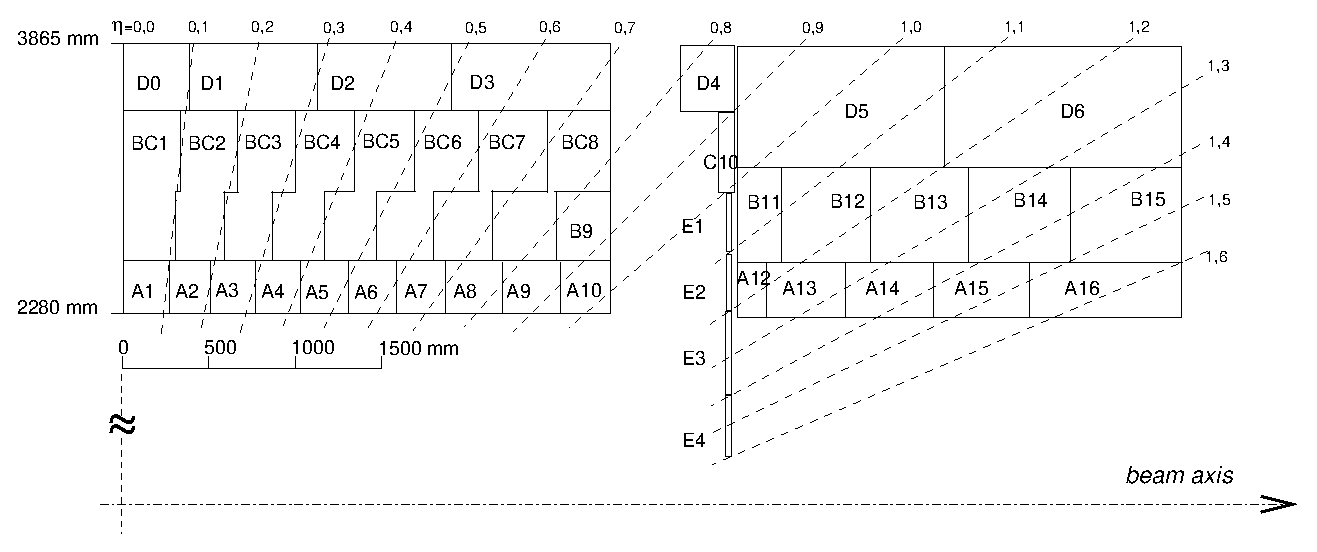
\includegraphics[width=\textwidth]{ATLASdetector/Figures/TileCal_Cells_and_Rows2}
  \end{center}
  \caption{Layout and geometry of the cells and layers in the hadronic calorimeter.}
  \label{fig:TileCalLayout}
\end{figure}

The author has contributed to performance studies of the hadronic calorimeter, and the work has been documented in appendix~\ref{chapter:TileTimingPerformance}.
\newline

The Hadronic End-Cap calorimeter (HEC) uses copper as passive material and liquid argon as active material, chosen for its radiation hardness in a region ($1.5 < \abseta < 3.2$) exposed to a significant particle flux.
  Each HEC is composed of two independent wheels with granularity varying with $\eta$.
In $1.5 < \abseta < 2.5$, $\Delta \eta \times \Delta \phi = 0.1 \times 0.1$ in the first two longitudinal layers, and $0.2\times0.1$ in the last one.
In the range $2.5 < \abseta < 3.2$, the granularity is $\Delta \eta \times \Delta \phi = 0.2 \times 0.2$ in all the three samples.

Finally, the Forward Calorimeter (FCal) covers the very forward region of pseudorapidity, $3.1 < \abseta < 4.9$, making the calorimeter system achieve its good hermeticity and minimizing the energy losses.
It is assembled with tungsten rod absorbers embedded in a copper matrix.
Between the two, a thin gap filled with liquid argon provides the active material.


\subsection{Muon spectrometers}
    \label{subsec:MuonSpectrometers}

    The most external detector system is the muon spectrometer~\cite{MUONtdr}, a combination of toroidal superconducting magnets and precision chambers providing a measurement of the momentum of muons for $\abseta < 2.7$.
    %, in addition to the measurement from the ID.
    It is also equipped with an independent trigger system used for the first event triggering stage (see section~\ref{sec:TriggerSystem}) active in the pseudorapidity region $\abseta < 2.4$.
    Four subdetectors compose the muon system: Monitored Drift-Tube (MDT) chambers, Cathode Strips Chambers (CSC), Resistive Plate Chambers (RPC) and Thin Gap Chambers (TGC).
The layout changes in the barrel and end-cap regions, and is schematically shown in figure~\ref{fig:MuonSpectrometerSchema}.
In the barrel region, chambers are arranged in three cylindrical layers around the beam axis, one layer being inside the magnet.
In the end-caps these three layers are placed perpendicular to the beam axis.
The variety of technologies used responds to the different needs of the detector (precise position and momentum measurement versus triggering and time measurement) and the large variation in particle flux from the central to the forward region.

\begin{figure}[!tb]
  \begin{center}
      \includegraphics[width=0.7\textwidth]{ATLASdetector/Figures/MuonSystem.eps}
  \end{center}
  \caption{Schematic view of the ATLAS muon spectrometer.}
  \label{fig:MuonSpectrometerSchema}
\end{figure}

\subsubsection{Detection chambers}

\begin{description}
  \item[MDT] (Monitored Drift Tube chambers): 
    MDTs are proportional chambers based on pressurized drift tubes filled with an argon and carbon dioxide mixture and with a tungsten-rhenium wire producing a radial electric field.
%    made of aluminium with a diameter of \unit[30]{mm} and length varying from \unit[0.9]{m} to \unit[6.2]{m}.
%The gas mixture in them is 93\% Ar and 7\% $\text{CO}_2$, the anode is a $\unit[50]{\mu m}$ tungsten-rhenium wire producing a radial electric field.
Each chamber is composed of a group of six or eight tubes placed transverse to the beam axis.
This number of tubes allows for a very good track reconstruction and high reduction of the fake tracks from random associations of background hits, providing a resolution on position of $\unit[80]{\mu m}$ for an individual tube, $\unit[40]{\mu m}$ for a chamber and $\unit[30]{\mu m}$ for the three layers of MDTs.
    Due to their reliability, mechanical robustness and simpler operation, MDT chambers are employed to cover the larger area of the spectrometer ($\abseta <2.7$, $2.0$ for the innermost layer).
%The basic detection element is a cylindrical aluminum drift tube filled with gas and a central wire at a high potential.
%The muons passing through the tubes ionize the gas and produce charges that are collected on the wire.

  \item[CSC] (Cathode Strip Chambers): CSCs are multiwire proportional chambers with wires oriented in the radial direction, spaced by \unit[2.5]{mm}, and using the same gas mixture as the MDTs.
%The cathode strips are oriented, one perpendicularly to the anode wires (and gives the precision coordinate), and the other parallel to the wires (and gives the transverse coordinate).
  CSCs are used at high pseudo-rapidities to help confront the demanding rate and background conditions.
%They are arranged in a system of two disks with eight chambers each.
%Each chamber contains four multiwire proportional chambers (the CSCs)
%    The spatial resolution provided by one individual chamber is $\sim \unit[60]{\mu m}$.
    The spacial resolution of the four layers of CSCs is $\unit[40]{\mu m}$ in the bending plane and $\unit[5]{mm}$ in the non-bending one.
    The maximum drift time for signal collection is \unit[40]{ns} compared to the \unit[700]{ns} of the MDTs, which gives the possibility to achieve higher acquisition rates.
Due to this capability, together with the high radiation resistance, CSCs are used in the range $2.0 < \abseta < 2.7$.
\end{description}

\subsubsection{Triggering chambers}

For trigger purposes detectors with faster response than drift tubes are needed,\footnote{Drift-time in tubes with a diameter of $\sim \unit[10]{mm}$ can be of $\sim \unit[500]{ns}$, too long with respect to the \unit[25]{ns} spacing of the bunch crossings.}
MDTs and CSCs are therefore supplemented with special layers of trigger chambers.

\begin{description}
  \item[RPC] (Resistive Plate Chambers): RPCs are chambers with a gas mixture of $\text{C}_2\text{H}_2\text{F}_4$ (94.7\%), Iso-$\text{C}_4\text{H}_{10}$ (5\%) and $\text{SF}_6$ (0.3\%) between two resistive Bakelite plates.
    %separated by \unit[2]{mm} and containing a .
The avalanches are collected with two orthogonal sets of pick-up strips that provides a position resolution of \unit[1]{cm} in each plane and \unit[1]{ns} time resolution, allowing for individual bunch crossing discrimination.
RPCs provide also the $\phi$ coordinate for the tracks in the final analysis, since MDTs only give the $\eta$ coordinate.

  \item[TGC] (Thin Gap Chamber): TGCs are multi-wire proportional chambers with the characteristic that the wire-to-cathode distance is smaller than the wire-to-wire distance for a fast collecting time.
They are assembled in the end-cap wheels, covering the region $1.05 < \abseta < 2.7$ (2.4 for triggering).
The timing resolution is comparable to the RPC's one while the spatial resolution is in the range of \unit[2-7]{mm} for both coordinates.
\end{description}


\section{Forward subdetectors and luminosity measurement}
    \label{sec:LuminosityMeasurement}
    
A good determination of the integrated luminosity is of particular importance to reach the ultimate precision in measurement of processes of interest.
The luminosity, $\InstLumi$, defined in equation~\ref{eq:InstLumiDefinition}, can be rewritten as:
\begin{equation}
  \InstLumi = \frac{\mu_{\mathrm{vis}}n_b f_r}{\sigma_{\mathrm{vis}}}~,
\end{equation}
where $f_r$ is the collider revolution frequency, $n_b$ the number of colliding bunches
and $\sigma_{\mathrm{vis}}$ the visible inelastic \xsec\ (total inelastic \xsec\ times the detector acceptance and efficiency).
The  visible interaction rate per bunch crossing is denoted as $\mu_{\mathrm{vis}}$.
It is extracted mainly from the signals coming from specific luminosity detectors.
The simplest algorithm consists in ``simple counting'' of bunch crossings where detectors reported a signal, but more refined algorithms~\cite{Aad:2013ucp} are used,
in particular when the \pileup\ contamination is no longer negligible.

In order to use the measured $\mu_{\mathrm{vis}}$ for luminosity determination, 
each detector and algorithm must be calibrated by determining its
visible \xsec\ $\sigma_{\mathrm{vis}}$.
The calibration technique exploits the \textit{van der Meer}
scans~\cite{vdMscan}.
These are special low-intensity LHC 
runs where the beam separation in the transverse planes  is varied (scanned) in order to determine 
the beams' overlap profile.
Through the determination of the beam lateral profile the absolute luminosity of the particular run can be inferred using formula~\ref{eq:InstLumiDefinition}, and $\sigma_{\mathrm{vis}}$ can be determined for each subdetector.

    ATLAS is supplemented with several detectors in the forward regions to perform luminosity measurements and monitoring.
The main detectors for luminosity measurement are listed below:
\begin{description} 
%  \item[MBTS] (Minimum Bias Trigger Scintillators): located at $z = \pm \unit[365]{cm}$ from the interaction point, they cover the pseudorapidity region {$2.09<\abseta < 3.84$}.
%The MBTS were employed during 2010 to trigger on events with minimal requirement on collision activity.
%During 2011 and 2012, they were not considered as luminosity detectors given the saturation effect produced by the high interaction rate.
\item[LUCID] (LUminosity measurements using Cherenkov Integrating Detector): a Cherenkov detector specifically designed for luminosity measurement.
It consists of 16 aluminum tubes surrounding the beam pipe at \unit[17]{m} from the interaction point.
Each tube is filled with 
$\mathrm{C}_4\mathrm{F}_{10}$ and is coupled to a photomultiplier in the back-end.
\item[BCM] (Beam Conditions Monitor): $\unit[1]{cm^2}$ diamond detectors located at $z = \pm\unit[184]{cm}$ around the beam pipe.
  Their fast readout and good time resolution (\unit[0.7]{ps}) allow them to provide luminosity information for each bunch crossing.
At the same time they are also employed to trigger on beam losses and induce the dump of the beam, thus protecting the silicon detectors from damage that might result from an uncontrolled beam.

\item[ALFA] (Absolute Luminosity For ATLAS): is a subdetector that is only activated during special runs.
It consists of  8 scintillating fibers detectors placed at \unit[240]{m} from the interaction point inside roman pots, above and below the beam pipe.
\end{description}

In addition, cross-checks of the luminosity measurement have been performed using information from other standard subdetectors:
counting of primary vertices reconstructed by the ID and integrated signals from the Tile and forward calorimeter.
The precision achieved is of a few \% depending on the data-taking year.
\section{Trigger system}
    \label{sec:TriggerSystem}

    Due to technical limitations, not every LHC collision can be recorded by the ATLAS detector.
    The goal of the ATLAS trigger and data acquisition system is to select in real time events with interesting characteristics for physics analyses.
%The purpose of the trigger system is to reduce the input rate from several MHz to about $\unit[400]{Hz}$ for recording and offline processing.
%This limit is equivalent to an average data rate of about $\unit[300]{MB/s}$, which is the maximum that the computer resources and the offline storage can handle.
%For each bunch crossing, the trigger system verifies if at least one of hundreds of conditions (triggers) are satisfied.
%Most of them are based on identifying combinations of candidate physics objects such as electrons, muons or jets, but there are also triggers for inelastic $\pp$ collisions (minimum bias) and triggers based on global event properties, such as $\sum\et$ or $\met$.

\begin{figure}[!tb]
  \begin{center}
      \includegraphics[width=0.55\textwidth]{ATLASdetector/Figures/TriggerSystem.eps}
  \end{center}
  \caption[Schema of the ATLAS trigger system.]{Schema of the ATLAS trigger system.}
  \label{fig:TriggerSchema}
\end{figure}

The ATLAS trigger system~\cite{Aad:2012xs}, shown schematically in figure~\ref{fig:TriggerSchema}, has a three-layer structure with increasingly detailed levels of information used in the reconstruction, and hence refinement of the selection criteria at each stage.

% \subsection{Level 1 trigger}
% \label{L1}

At the first stage, Level 1 (L1), hardware triggers use coarse calorimeter and muon information for the trigger decision.
At this level the event rate is reduced from \unit[40]{MHz} (the frequency of the beam crossing) to a maximum of \unit[75]{kHz}.
In the cases where the trigger is passed, the L1 trigger defines one or more regions-of-interest (RoIs) in $\eta$ and $\phi$ where the trigger has identified interesting features. The raw event data is then sent to the readout stream for the next trigger level.

The Level 2 (L2) trigger is based on software.
At this stage the information from the trackers is incorporated to the RoI to build candidate objects (electrons, photons, muons) and their position and energy are computed. A tighter selection on these refined objects allows for a reduction of the throughput down to $\approx \unit[3]{kHz}$.

The final trigger level is the Event Filter (EF).
The combination of the two software steps, L2 and EF, is referred to as High Level Trigger (HLT).
At this point the physics objects are built using the same algorithms as the offline reconstruction. After the selection, the EF reduces the output rate to \unit[200]{Hz} and the events are written to mass storage.
Events passing the EF are assigned to streams defined to separate the events into different datasets for different analysis' interests, e.g. electron streams, muon streams, jet streams, etc.

Most of the trigger chains used for physics are un-scaled, meaning that all the events passing the selection are kept. 
Other trigger chains that contain either too many events
or events considered not physically interesting are pre-scaled. 
These are characterized by a prescaling value, $P$, meaning that of all the events that activated
the trigger, only $1/P$ were accepted.
These trigger chains are usually used for checks or calibration rather than physics analysis.

The term ``trigger chain'' refers to the sequence of selections
that define a certain trigger object. The naming convention is:
\begin{equation*}\label{eq:}
  {\rm [LEVEL][N][TYPE(S)][THRESHOLD][ISOLATION][QUALITY]},
  \end{equation*}
  where the components, from left to right, are: the trigger level used, the
  multiplicity of the type, the object candidate, the threshold applied to
  the transverse momentum or energy of the object candidate, the object isolation and
  the severity of the final algorithm requirements.

  Trigger chains define a {\it trigger menu}, where they are associated to their
  prescale value $P$, and which is chosen based on the physics program of the
  data-taking period, taking into account the LHC luminosity.

%During the course of 2011 the RoI-seeded approach at the EF was replaced by a full-scan strategy.
%It was found that sufficient time was available to read the information from the entire ATLAS calorimetry system, which improves the online selection efficiency.

\section{Data quality}
\label{sec:DataQuality}
Not all collision events recorded by ATLAS are used for data analysis.
Each subdetector maintains a record of its performance across the run, and only the data collected with the subdetectors meeting certain quality requirements are considered for the analysis.
Therefore, for each dataset Good Runs Lists (GRL) are compiled recording for each lumiblock\footnote{
A luminosity block (lumiblock) is the smallest unit of time in the ATLAS data-taking defined as the minimal period where all the data-taking configurations are constant. In general the duration of a luminosity block is of the order of 1 minute.} 
which subdetectors satisfied the requirements.
For the measurements presented in this dissertation, all ATLAS subsystems are needed, as the physics objects used in the analyses are reconstructed using the information from the full detector.
The fraction of data considered as ``good'' is $\sim 95\%$, giving a total integrated luminosity of $\unit[20.3]{fb^{-1}}$ satisfying data quality that is used for these analyses.

\clearpage
\bibliographystyle{Bibliography/atlasnote}
\bibliography{Bibliography/myBib}
